% !TeX spellcheck = es_ES
% !TEX encoding = UTF-8 Unicode
\documentclass[t, compress, spanish, aspectratio=169]{beamer}
%\documentclass[t, compress, spanish]{beamer} % for the presentation
%\documentclass[handout]{beamer}    % for the handout

\usetheme[progressbar=frametitle]{metropolis}

%\usetheme[secheader]{Madrid}
%\usetheme{Frankfurt}
%\usetheme{Warsaw}
%\usetheme{Berlin}
%\usetheme{CambridgeUS}

%\usecolortheme{beaver}     % Fondo Blanco y letras Negras - Titulos en Rojo con fondo gris
%\usecolortheme{dove}       % Para el Handout
%\usecolortheme{seahorse}   % Fondo Blanco y letras Negras - Titulos en Celeste
%\usecolortheme{dolphin}    % Fondo Blanco y letras Negras - Titulos en Celeste
%\usecolortheme{seagull}    % Fondo Blanco y letras Negras - Titulos en Gris
%\usecolortheme{crane}      % Fondo Blanco y letras Negras - Titulos en Amarillo
%\usecolortheme{wolverine}  % Fondo Blanco y Letras negras - Titulos en negro con fondo amarillo
%\usecolortheme{lily}       % Fondo Blanco y letras Negras - Titulos en Azul
%\usecolortheme{fly}        % Fondo Gris y letras Negras - Titulos en Rojo
%\usecolortheme{beetle}     % Fondo Gris y letras Negras - Titulos en blanco
%\usecolortheme{albatross}  % Fondo Azul y letras blancas
%\usecolortheme{orchid}     % Default
%\usecolortheme{rose}       % Default
%\usecolortheme{whale}      % Default

\setbeamertemplate{navigation symbols}{} % Gets rid of navigation symbols
%\setbeamercovered{transparent}

\usepackage{dsfont} % Double stroke fonts for math symbols
% \usepackage[T1]{fontenc}  % Helps with hyphenation for languages with accented characters. Note: Does not work with XeLaTex
% \usepackage[latin1]{inputenc} % Allows to type in latin (accents). Note: Does not work with XeLaTex
% \usefonttheme[onlymath]{serif}  % Changes fonts for math to serif
\usepackage[english]{babel} % Manages differences between languages: hyphenation etc

\usepackage{appendixnumberbeamer} % Does not include backup slides in the number of pages

\usepackage{centernot} % To draw not in math symbols (does not imply)

\usepackage{ragged2e}  % Text alignment
\justifying

\usepackage{graphicx} % Format for graphics: additional options for includefigure
\usepackage{pgf} % Tool for graphics
\usepackage{pgfplots} % Plotting on top of tikz/pgf
\pgfplotsset{compat=1.17}

\usepackage{booktabs} % Format for tables: top, bottom and mid lines
\usepackage[scale=2]{ccicons}
\usepackage{threeparttable} % Format for tables
\usepackage{lscape} % Landscape for tables

% Customized commands
  \newcommand{\vs}{\vskip0pt plus.5fill}
  \newcommand{\SR}{\mathbb{R}}
  \DeclareMathOperator{\plim}{plim}
  \DeclareMathOperator{\Var}{Var}
  \DeclareMathOperator{\Avar}{AVar}
  \DeclareMathOperator{\Cov}{Cov}
  \DeclareMathOperator{\N}{Normal}
  \DeclareMathOperator{\E}{\mathbb{E}}
  \DeclareMathOperator{\LP}{\mathbb{L}}
  \newcommand{\pto}{\stackrel{p}{\longrightarrow}}
  \newcommand{\dto}{\stackrel{d}{\longrightarrow}}
  \newcommand{\adistr}{\stackrel{a}{\sim}}
  \newcommand{\epsi}{\varepsilon}
  \newcommand{\tmle}{\hat \theta_{ML}}
  \newcommand{\tgmm}{\hat \theta_{GMM}}
  \newcommand\independent{\protect\mathpalette{\protect\independenT}{\perp}}
  \def\independenT#1#2{\mathrel{\rlap{$#1#2$}\mkern2mu{#1#2}}}
  \newcommand{\term}[1]{\structure{\textbf{#1}}} % label/definition markup, distinct from \alert (reserved for genuine callouts)


\title [Teor\'ia asint\'otica] {An\'alisis Econom\'etrico\\
	Teor\'ia Asint\'otica}
\author[de Elejalde]{Ramiro de Elejalde}
\institute [UAH] {Facultad de Econom\'ia y Finanzas \\ Universidad Alberto Hurtado}
\date[\today] {}
\subject{An\'alisis Econom\'etrico}
\begin{document}
	
	%------------------------------------------------------------
	
	\begin{frame}
		\titlepage
	\end{frame}
	
	% --------------------------------------------------- Slide --
	\begin{frame}
		\frametitle{Outline}
		\footnotesize
		\tableofcontents
		\alert{Referencias}: Cap. 7 y 8 Hansen (Introduction to Econometrics), y cap. 3 de Wooldridge.
	\end{frame}
	
	% --------------------------------------------------- Slide --
	\begin{frame}
		\frametitle{Estimador}
		\begin{itemize}
			\item Dada una muestra aleatoria podemos calcular un estimador para ``aproximar'' los  par\'ametros poblacionales de inter\'es.
			\item Nos interesa que el estimador tenga ``buenas'' propiedades.
			\item En este curso nos enfocamos en las propiedades del estimador cuando $N\to \infty$, las \term{propiedades asint\'oticas}.
			% MCO es insesgado, pero no tiene varianza minima excepto en casos especiales de poco inter\'es (homoscedasticidad). Adem\'as, no conocemos su distribuci\'on pra cualquier N excepto en casos particulares como con inobservado normal. IV no es siquiera insesgado.
			\begin{enumerate}
				\item Cuando $N$ crece, la distribuci\'on del estimador se concentra alrededor del par\'ametro (\term{consistencia})
				\item Cuando $N$ crece la distribuci\'on del estimador (estandarizada) se acerca a una distribuci\'on normal (\term{distribuci\'on asint\'otica normal})
			\end{enumerate}
			\item En esta unidad vamos a estudiar teoremas que nos permitan obtener las propiedades asint\'oticas de los estimadores que vamos a estudiar durante el curso.
		\end{itemize}
	\end{frame}		

	\section{Propiedades en muestras peque\~nas de los estimadores}

    \begin{frame} 
        \frametitle{Repaso de estad\'istica}      
        \begin{itemize}
    		\item <1->\term{Par\'ametro}: Caracter\'istica de la poblaci\'on de inter\'es. Ejemplo: $\mu=\E(y)$
    		\item <2-> \term{Muestra aleatoria}: Muestra de tama\~no $N$ de la poblaci\'on obtenida en forma aleatoria y con reemplazo $\{y_1,y_2,...,y_N\}$. \\
		El muestreo aleatorio nos asegura que $y_1, y_2, ...,y_N$ se distribuyen i.i.d.
    		\item <3-> \term{Estimador}:  Un estad\'istico (funci\'on de las variables muestrales) que se utiliza para estimar un par\'ametro de inter\'es. Ejemplo: Media muestral $\bar y = \frac{1}{N}\sum_{i=1}^{N} y_i$.
    		\item <4-> Recordar las propiedades de la varianza $\Var(y)$
    		\begin{itemize}
    			\item $\Var(a+bx)=b^2\Var(x)$
    			\item $\Var(bx+cy)=b^2\Var(x)+c^2\Var(y)+2 bc\Cov(x,y)$
    		\end{itemize}        
    	\end{itemize}     
    \end{frame}    
	
	\begin{frame}
		\frametitle{Propiedades en muestras peque\~nas de los estimadores}
		\begin{itemize}
			\item <1->\term{Insesgadez}: Un estimador $\hat \theta_N$ de un par\'ametro $\theta$ es \term{insesgado} si,
			\begin{align*}
			\E(\hat \theta_N) = \theta \text{ para todo }N.
			\end{align*}
		\end{itemize}
	\end{frame}

	\begin{frame}
		\frametitle{Propiedades en muestras peque\~nas de los estimadores}
		\begin{itemize}
			\item <1->\term{Eficiencia}: Un estimador $\hat \theta_N$ de un par\'ametro $\theta$ es \term{eficiente} si,
			\begin{align*}
			\Var(\hat \theta_N) \leq \Var(\tilde \theta_N),
			\end{align*}
			para todo $\tilde \theta_N$ en una familia de estimadores de $\theta$ con ciertas propiedades (por ejemplo, insesgados y lineales).
		\end{itemize}
	\end{frame}
	
	\begin{frame}
		\frametitle{Ejemplo: Media muestral}
		\begin{itemize}
			\item Dada una muestra i.i.d. $\{y_1,...,y_N\}$ con $\E(y_i)=\mu$ y $\Var(y_i)=\sigma^2$
			\item Par\'ametro: $\mu$.
			\item Estimador: \term{media muestral}
			\begin{align*}
			\bar y = \frac{1}{N} \sum_i y_i.
			\end{align*}
		\end{itemize}
	\end{frame}

	\begin{frame}
		\frametitle{Ejemplo: Media muestral}
		\begin{itemize}
			\item Insesgadez: $\E(\bar y)=\mu$
		\end{itemize}
	\end{frame}

	\begin{frame}
		\frametitle{Ejemplo: Media muestral}
		\begin{itemize}
			\item [] Soluci\'on: Por linealidad de la esperanza,
			\begin{align*}
			\E(\bar y) = \E\left(\frac{1}{N}\sum_i y_i\right) = \frac{1}{N}\sum_i \E(y_i) = \frac{1}{N}(N\mu) = \mu.
			\end{align*}
		\end{itemize}
	\end{frame}

	\begin{frame}
		\frametitle{Ejemplo: Media muestral}
		\begin{itemize}
			\item Eficiencia: $\Var(\bar y)=\frac{\sigma^2}{N}$
		\end{itemize}
	\end{frame}

	\begin{frame}
		\frametitle{Ejemplo: Media muestral}
		\begin{itemize}
			\item [] Soluci\'on:
			\begin{align*}
			\Var(\bar y) = \Var\left(\frac{1}{N}\sum_i y_i\right) = \frac{1}{N^2}\sum_i \Var(y_i) = \frac{1}{N^2}(N\sigma^2) = \frac{\sigma^2}{N},
			\end{align*}
			donde usamos independencia ($\Cov(y_i,y_j)=0$ para $i\neq j$) y que las $y_i$ son id\'enticamente distribuidas ($\Var(y_i)=\sigma^2$ para todo $i$).
		\end{itemize}
	\end{frame}


	% --------------------------------------------------- Slide --
	\section{Propiedades asint\'oticas de los estimadores}
	\begin{frame}
		\frametitle{Convergencia de variables aleatorias}
		\begin{itemize}			
			\item El an\'alisis asint\'otico se ocupa de estudiar la \term{convergencia de una secuencia de variables aleatorias}. 
			\item Cuando aplicamos estos conceptos a econometr\'ia, las variables aleatorias son estimadores cuya distribuci\'on depende del tama\~no de la muestra $N$ y buscamos la distribuci\'on del estimador cuando $N \to \infty$.
		\end{itemize}
	\end{frame}
	
	\begin{frame}
		\frametitle{Ejemplos}
		\begin{itemize}
				\item Una secuencia determin\'istica puede ser $\{a_N\}_{N=1}^{\infty}$ donde $a_N=\{2+\frac{1}{N}\}$.
		\end{itemize}
		\begin{center}
			\begin{tikzpicture}
				\begin{axis}[
					width=0.85\textwidth, height=5.2cm,
					xlabel={$N$}, ylabel={$a_N$},
					xlabel style={font=\small}, ylabel style={font=\small},
					tick label style={font=\small},
					xmin=0, xmax=30, ymin=1.9, ymax=3.1,
					]
					\addplot[only marks, mark=*, mark size=1.3pt, blue, domain=1:30, samples=30] {2+1/x};
					\addplot[dashed, thick, red, domain=0:30, samples=2] {2};
				\end{axis}
			\end{tikzpicture}
		\end{center}
	\end{frame}

	\begin{frame}
		\frametitle{Ejemplos}
		\begin{itemize}
				\item Una secuencia de variables aleatorias puede ser
				\begin{align*}
				z_N=\left\{
				\begin{array} {l l}
				0 & \text{con probabilidad } 1-\frac{1}{N}, \\
				N & \text{con probabilidad } \frac{1}{N},
				\end{array}
				\right.
				\end{align*}
		\end{itemize}
		\begin{center}
			\begin{tikzpicture}
				\begin{axis}[ybar, width=4.6cm, height=4.2cm, title={$N=1$}, title style={font=\small},
					ylabel={densidad}, ylabel style={font=\small}, tick label style={font=\small},
					ymin=0, ymax=1.15, xtick={0,1}, bar width=12pt]
					\addplot coordinates {(0,0) (1,1)};
				\end{axis}
			\end{tikzpicture}
			\begin{tikzpicture}
				\begin{axis}[ybar, width=4.6cm, height=4.2cm, title={$N=2$}, title style={font=\small},
					tick label style={font=\small},
					ymin=0, ymax=1.15, xtick={0,2}, bar width=12pt]
					\addplot coordinates {(0,0.5) (2,0.5)};
				\end{axis}
			\end{tikzpicture}
			\begin{tikzpicture}
				\begin{axis}[ybar, width=4.6cm, height=4.2cm, title={$N=3$}, title style={font=\small},
					tick label style={font=\small},
					ymin=0, ymax=1.15, xtick={0,3}, bar width=12pt]
					\addplot coordinates {(0,0.667) (3,0.333)};
				\end{axis}
			\end{tikzpicture}
		\end{center}
	\end{frame}


	\begin{frame}
		\frametitle{Ejemplos}
		\footnotesize
		La media muestral para una muestra de tama\~no $N$: $\bar y_N$. La secuencia es $\{\bar y_1, \bar y_2,...\}$ -- por ejemplo, para $y_i\sim$ Bernoulli($p=0.78$):
		\vspace{-.20cm}
		\begin{center}
			
\includegraphics[width=0.28\textwidth]{figures/sample_mean2.png}
			
\includegraphics[width=0.28\textwidth]{figures/sample_mean5.png}
		\end{center}
		\vspace{-.3cm}
		\begin{center}
			
\includegraphics[width=0.28\textwidth]{figures/sample_mean25.png}
			
\includegraphics[width=0.28\textwidth]{figures/sample_mean100.png}
		\end{center}
	\end{frame}
	

	% --------------------------------------------------- Slide --
	\subsection{Convergencia en probabilidad}
	\begin{frame}
		\frametitle{Convergencia para secuencias determin\'isticas}
		\begin{itemize}
			\item Una secuencia determin\'istica $a_N$  \term{converge} a $a$ cuando $N \to \infty$ si para todo $\delta>0$ existe $N_\delta < \infty$ tal que,
			\begin{align*}
			|a_N-a|\leq \delta \quad  \text{ para todo } N\geq N_\delta.
			\end{align*}
			\item Notaci\'on: $a_N \to a$ \'o $\lim a_N=a$
		\end{itemize}
	\end{frame}

	\begin{frame}
		\frametitle{Convergencia para secuencias determin\'isticas}
		\begin{itemize}
			\item \term{Ejemplo}: La secuencia determin\'istica $\{a_N\}_{N=1}^{\infty}$ donde $a_N=\{2+\frac{1}{N}\}$ converge a $\lim_{N\to \infty } a_N=2$.
			\item [] Soluci\'on formal: Dado $\delta>0$, sea $N_\delta=1/\delta$. Para todo $N\geq N_\delta$,
			\begin{align*}
			|a_N-2|=\left|\frac{1}{N}\right|=\frac{1}{N}\leq \frac{1}{N_\delta}=\delta.
			\end{align*}
			Por lo tanto $a_N\to 2$.
		\end{itemize}
	\end{frame}

	\begin{frame}
		\frametitle{Convergencia en probabilidad}
		\begin{itemize}
			\item Una variable aleatoria $z_N$ \term{converge en probabilidad} a una constante $c$ cuando $N \to \infty$ si para todo $\delta>0$,
			\begin{align*}
			\lim_{N\to \infty }\Pr(|z_N-c|\leq \delta)=1
			\end{align*}
			\item Notaci\'on: $z_N \pto c$ \'o $\plim z_N=c$
		\end{itemize}
	\end{frame}
	
	
	\begin{frame}
		\frametitle{Convergencia en probabilidad}
		\begin{itemize}
			\item\term{Ejemplo}: Calcule la convergencia en probabilidad de $z_N$
			\begin{align*}
			z_N=\left\{ 
			\begin{array} {l l}
			0 & \text{con probabilidad } 1-\frac{1}{N}, \\
			N & \text{con probabilidad } \frac{1}{N},
			\end{array}
			\right.
			\end{align*}
%			\item <4->\alert{?`Convergencia en probabilidad es lo mismo que convergencia de la media? }$\lim_{N\to\infty}\E(z_N)=c$?
%			\uncover<5-> {Respuesta: No, en el ejemplo $\lim_{N\to\infty}\E(z_N)=1\neq 0$.}
		\end{itemize}
	\end{frame}
	
	
	\begin{frame}
		\frametitle{Convergencia en probabilidad}
		\begin{itemize}
			\item\term{Ejemplo}: Calcule la convergencia en probabilidad de $z_N$
			\begin{align*}
			z_N=\left\{ 
			\begin{array} {l l}
			0 & \text{con probabilidad } 1-\frac{1}{N}, \\
			N & \text{con probabilidad } \frac{1}{N},
			\end{array}
			\right.
			\end{align*}
			\item {Respuesta: $z_N \pto 0$.}
			\item [] Soluci\'on formal: Dado $\delta>0$, para $N>\delta$ se tiene $\{z_N=N\}\implies |z_N-0|>\delta$, por lo tanto
			\begin{align*}
			\Pr(|z_N-0|\leq \delta) = \Pr(z_N=0) = 1-\frac{1}{N} \xrightarrow[N\to\infty]{} 1.
			\end{align*}
			Como esto vale para todo $\delta>0$, $z_N \pto 0$.
%			\item <4->\alert{?`Convergencia en probabilidad es lo mismo que convergencia de la media? }$\lim_{N\to\infty}\E(z_N)=c$?
%			\uncover<5-> {Respuesta: No, en el ejemplo $\lim_{N\to\infty}\E(z_N)=1\neq 0$.}
		\end{itemize}
	\end{frame}


	% --------------------------------------------------- Slide --
	\subsection{Consistencia.}
	\begin{frame}
		\frametitle{Consistencia}
		\begin{itemize}
			\item  \term{Consistencia}: Un estimador $\hat \theta_N$ de un par\'ametro $\theta$ es \term{consistente} si,
			\begin{align*}
			\hat \theta_N \pto \theta \text{ cuando }N \to \infty.
			\end{align*}
		\end{itemize}
	\end{frame}
	
	% --------------------------------------------------- Slide --
	\begin{frame}
		\frametitle{Ejemplo: Bernoulli con p=0.78}
		\footnotesize
		Simulaci\'on: $y_i\sim$ Bernoulli($p=0.78$) i.i.d.; distribuci\'on muestral de $\bar y_N$ para $N=2,5,25,100$. Al crecer $N$, se concentra alrededor de $p=0.78$ (consistencia).
		\vspace{-.20cm}
		\begin{center}
			
\includegraphics[width=0.28\textwidth]{figures/sample_mean2.png}
			
\includegraphics[width=0.28\textwidth]{figures/sample_mean5.png}
		\end{center}
		\vspace{-.3cm}
		\begin{center}
			
\includegraphics[width=0.28\textwidth]{figures/sample_mean25.png}
			
\includegraphics[width=0.28\textwidth]{figures/sample_mean100.png}
		\end{center}
	\end{frame}

	% --------------------------------------------------- Slide --
	\subsection{Ley (d\'ebil) de los grandes n\'umeros (LGN)}
	\begin{frame}
		\frametitle{Ley (d\'ebil) de los grandes n\'umeros (LGN)}
		\begin{itemize}
			%            \note[item]{Si $z_N$ es una media de variables aleatorias, ciertos teoremas nos ayudan.}
			
			\item <1->Dada una muestra i.i.d. de tama\~no $N$, si $\E|y|<\infty$, entonces cuando $N \to \infty$,
			\begin{align*}
			\frac{1}{N} \sum_{i=1}^N y_i\pto \E(y).
			\end{align*}
			%            \note[item]{WLLN: (Proof) Desigualdad de Chebycheff $\Pr(|\bar y - \mu| > \epsilon) \leq \frac{\sigma^2/N}{\epsilon}$}
			
			\item <2-> Extensi\'on para vectores aleatorios. Definimos a $\mathbf{y}: \SR^m \times 1$. Dada una muestra i.i.d. de tama\~no $N$, si $\E|\mathbf{y}|<\infty$, entonces cuando $N \to \infty$,
			\begin{align*}
			\frac{1}{N} \sum_{i=1}^N \mathbf{y}_i\pto \E(\mathbf{y}).
			\end{align*}
		\end{itemize}
	\end{frame}
	
	% --------------------------------------------------- Slide --
	\begin{frame}
		\frametitle{Ejemplos}
		\begin{itemize}
			\item \term{Media muestral}
			\begin{align*}
			\bar y = \frac{1}{N}\sum_{i=1}^N y_i \pto \mu
			\end{align*}
			donde $\mu=\E(y)$.
		\end{itemize}
	\end{frame}

	\begin{frame}
		\frametitle{Ejemplos: soluci\'on}
		\begin{itemize}
			\item [] Soluci\'on: Aplicando la LGN a la muestra i.i.d. $\{y_i\}$,
			\begin{align*}
			\bar y = \frac{1}{N}\sum_{i=1}^N y_i \pto \E(y) = \mu.
			\end{align*}
		\end{itemize}
	\end{frame}


	% --------------------------------------------------- Slide --
	\begin{frame}
		\frametitle{Ejemplos}
		\begin{itemize}
			\item \term{Media muestral de $y_i^2$}
			\begin{align*}
			\frac{1}{N}\sum_{i=1}^N y_i^2 \pto \E(y^2)
			\end{align*}
		\end{itemize}
	\end{frame}

	\begin{frame}
		\frametitle{Ejemplos: soluci\'on}
		\begin{itemize}
			\item [] Soluci\'on: $\{y_i^2\}$ tambi\'en es una muestra i.i.d. (funci\'on de una muestra i.i.d.). Aplicando la LGN a $\{y_i^2\}$,
			\begin{align*}
			\frac{1}{N}\sum_{i=1}^N y_i^2 \pto \E(y^2).
			\end{align*}
		\end{itemize}
	\end{frame}

	% --------------------------------------------------- Slide --
	\subsection{Teorema de la funci\'on continua}
	\begin{frame}
		\frametitle{Teorema de la funci\'on continua}
		%        \note[item] {?`Qu\'e pasa cuando tenemos una funci\'on de medias como $S^2=\frac{1}{N} \sum_i y_i^2-\bar y^2 $? }
		\begin{itemize}
			\item Si $z_N \pto c$ cuando $N \to \infty$, y $g(.)$ es continua en $c$, entonces
			\begin{align*}
			g(z_N) \pto g(c) \text{ cuando }N \to \infty.
			\end{align*}
		\end{itemize}
	\end{frame}
	
	% --------------------------------------------------- Slide --
	\begin{frame}
		\frametitle{Ejemplos}
		\begin{itemize}
			\item \term{Varianza muestral}
			\begin{align*}
			S^2 &=\frac{1}{N}\sum_{i=1}^N (y_i-\bar y)^2 \\
			& = \frac{1}{N}\sum_{i=1}^N y_i^2-\bar y^2\pto \sigma^2,
			\end{align*}
			donde $\sigma^2=\Var(y)$.
		\end{itemize}
	\end{frame}

	\begin{frame}
		\frametitle{Ejemplos: soluci\'on}
		\begin{itemize}
			\item [] Soluci\'on: Por LGN, $\bar y \pto \mu$ y $\frac{1}{N}\sum_i y_i^2 \pto \E(y^2)$. La funci\'on $g(a,b)=a-b^2$ es continua, luego por el teorema de la funci\'on continua,
			\begin{align*}
			\frac{1}{N}\sum_i y_i^2-\bar y^2 = g\left(\frac{1}{N}\sum_i y_i^2,\, \bar y\right) \pto g(\E(y^2),\mu) = \E(y^2)-\mu^2 = \sigma^2.
			\end{align*}
		\end{itemize}
	\end{frame}

	% --------------------------------------------------- Slide --
	\begin{frame}
		\frametitle{Ejemplos}
		\begin{itemize}
			\item \term{Desviaci\'on est\'andar muestral:} $S \pto \sigma$
		\end{itemize}
	\end{frame}

	\begin{frame}
		\frametitle{Ejemplos: soluci\'on}
		\begin{itemize}
			\item [] Soluci\'on: Ya vimos $S^2\pto \sigma^2$. La funci\'on $g(x)=\sqrt{x}$ es continua para $x\geq 0$, luego por el teorema de la funci\'on continua,
			\begin{align*}
			S=\sqrt{S^2}=g(S^2)\pto g(\sigma^2)=\sqrt{\sigma^2}=\sigma.
			\end{align*}
		\end{itemize}
	\end{frame}


	% --------------------------------------------------- Slide --
	
	\begin{frame}
		\frametitle{Diferencias entre insesgadez y consistencia}
		\begin{itemize}
			\item <1->\term{Insesgadez no implica consistencia.} 
			\item [] <1-> Ejemplo: $\tilde y=y_1$
			\item <2->\term{Consistencia no implica insesgadez. }
			\item [] <2-> Ejemplo: Varianza muestral $S^2$
			\item <3->Teorema: Si $\lim_{N\to \infty} \E(\hat \theta_N)=\theta$ y $\lim_{N\to \infty}\Var(\hat \theta_N)=0$, entonces $\hat \theta_N \pto \theta \text{ cuando }N \to \infty$.
			\item <4->\term{Consistencia no implica insesgadez asint\'otica.}
			\item [] <5->Ejemplo donde consistencia no implica insesgadez asint\'otica: $z_N = 0$ con probabilidad $1-1/N$, y $z_N = N$ con probabilidad $1/N$.
		\end{itemize}
	\end{frame}

	%    \note[item]{Insesgadez no implica consistencia : Utilizar $y_1$ (primera observaci\'on de la muestra) como estimador de $\mu$.}
	%    \note[item]{Consistencia no implica insesgadez: Varianza muestral es sesgada pero consistente.}
	%    \note[item]{Consistencia no implica convergencia en media (insesgadez asint\'otica).}
	%    \note[item]{Ejemplo: $z_N = 0$ con prob $1-1/N$,y $z_N = a_N$ con prob $1/N$ . Es consistente, pero $\E z_N = a_N/N$ entonces para $a_N=N$ tenemos $\lim \E z_N = 1$.}


	\subsection{Convergencia en distribuci\'on}

	% --------------------------------------------------- Slide --
	\begin{frame}
		\frametitle{Convergencia en distribuci\'on}
		\begin{itemize}
			\item Dada una variable aleatoria con funci\'on de distribuci\'on $F_N(u) = \Pr(z_N \leq u)$.\\
			$z_N$ \term{converge en distribuci\'on} a $z$ cuando $N \to \infty$ si para todo $u$ en donde $F(u) = \Pr(z \leq u)$ es continua,
			\begin{align*}
			F_N(u) \to F(u) \text{ cuando }N \to \infty.
			\end{align*}
		\end{itemize}
	\end{frame}	
	
	% --------------------------------------------------- Slide --
	\begin{frame}
		\frametitle{Convergencia en distribuci\'on}
		\begin{itemize}
			\item Ejemplo: Demuestre que
			\begin{align*}
			F_N(u) = \frac{\exp(Nu)}{1+\exp(Nu)} \to F(u) = \left\{
				\begin{array} {l l}
					0 & \text{si } u < 0, \\
					1 & \text{si } u \geq 0.
				\end{array}
			\right.
			\end{align*}

			\begin{center}
			\begin{tikzpicture}
				\begin{axis}[
					width=0.78\textwidth, height=5.2cm,
					xlabel={$u$}, ylabel={$F_N(u)$},
					xlabel style={font=\small}, ylabel style={font=\small},
					tick label style={font=\small},
					xmin=-1, xmax=1, ymin=-0.05, ymax=1.05,
					legend pos=outer north east, legend style={font=\footnotesize},
					]
					\addplot[blue, domain=-1:1, samples=100] {exp(1*x)/(1+exp(1*x))};
					\addlegendentry{$N=1$}
					\addplot[orange, domain=-1:1, samples=100] {exp(5*x)/(1+exp(5*x))};
					\addlegendentry{$N=5$}
					\addplot[green!60!black, domain=-1:1, samples=100] {exp(10*x)/(1+exp(10*x))};
					\addlegendentry{$N=10$}
					\addplot[dashed, thick, black, forget plot] coordinates {(-1,0) (0,0)};
					\addplot[dashed, thick, black] coordinates {(0,1) (1,1)};
					\addlegendentry{$F(u)$}
					\addplot[only marks, mark=*, mark size=2pt, black, forget plot] coordinates {(0,1)};
					\addplot[only marks, mark=o, mark size=2pt, black, forget plot] coordinates {(0,0)};
				\end{axis}
			\end{tikzpicture}
			\end{center}
		\end{itemize}
	\end{frame}

	% --------------------------------------------------- Slide --
	\begin{frame}
		\frametitle{Convergencia en distribuci\'on: soluci\'on}
		\small
		\begin{itemize}
			\item Si $u>0$: $Nu\to\infty$, luego $\exp(Nu)\to\infty$ y
			\begin{align*}
			F_N(u)=\frac{1}{1+\exp(-Nu)}\to \frac{1}{1+0}=1.
			\end{align*}
			\item Si $u<0$: $Nu\to-\infty$, luego $\exp(Nu)\to 0$ y $F_N(u)\to \frac{0}{1+0}=0$.
			\item Si $u=0$: $F_N(0)=\frac{1}{2}$ para todo $N$, pero esto \term{no importa}: $u=0$ es un punto de discontinuidad de $F$ (salta de 0 a 1 ah\'i), y la definici\'on de convergencia en distribuci\'on s\'olo exige $F_N(u)\to F(u)$ en los puntos de continuidad de $F$.
			\item [] Por lo tanto $F_N(u)\to F(u)$ para todo $u\neq0$, es decir $z_N \dto z$ donde $z$ tiene distribuci\'on degenerada en $0$ (i.e. $z=0$ con probabilidad 1). Cuando el l\'imite es una constante, convergencia en distribuci\'on implica convergencia en probabilidad a esa misma constante (lo vemos formalmente en la pr\'oxima slide), as\'i que esto tambi\'en implica $z_N \pto 0$.
		\end{itemize}
	\end{frame}


		% --------------------------------------------------- Slide --
	\begin{frame}
		\frametitle{Convergencia en distribuci\'on}
		\begin{itemize}
			\item Dada una variable aleatoria con funci\'on de distribuci\'on $F_N(u) = \Pr(z_N \leq u)$.\\
			$z_N$ \term{converge en distribuci\'on} a $z$ cuando $N \to \infty$ si para todo $u$ en donde $F(u) = \Pr(z \leq u)$ es continua,
			\begin{align*}
			F_N(u) \to F(u) \text{ cuando }N \to \infty.
			\end{align*}
			\item Notaci\'on: $z_N \dto z$.
			\item <2->Convergencia en probabilidad implica convergencia en distribuci\'on: $z_N \pto z\implies z_N \dto z$.
			\item <3-> Si $z_N$ converge en distribuci\'on a una constante entonces $z_N$ converge en probabilidad a dicha constante: $z_N \dto c \implies z_N \pto c$
	
			%            \note [item] {Convergencia punto a punto entre funciones.}
			%            \note [item] {Graficar para normal}
			%            \note [item] {$z_N \pto z\implies z_N \pto z$}
			%            \note [item] {$z_N \dto c\implies z_N \pto c$ (convergence to a constant)}
		\end{itemize}
	\end{frame}
	% --------------------------------------------------- Slide --

	\begin{frame}
		\frametitle{Distribuci\'on asint\'otica normal}
		\begin{itemize}
			\item Un estimador $\hat \theta_N$ de un par\'ametro $\theta$ se distribuye \term{$\sqrt{N}$-asint\'oticamente normal} si,
			\begin{align*}
			\sqrt{N}(\hat \theta_N - \theta ) \dto \N(0,V),
			\end{align*}
			donde $V$ es la varianza asint\'otica de $\sqrt{N}(\hat \theta_N - \theta )$ y se denota $\Avar(\sqrt{N}(\hat \theta_N - \theta ))=V$.
		\end{itemize}
	\end{frame}
	
	\begin{frame}
		\frametitle{Distribuci\'on asint\'otica normal}
		\begin{itemize}
			\item <1-> Decimos $\hat \theta_N \adistr \N(\theta, V/N)$ donde $\Avar(\hat \theta_N)=V/N$ es la \term{varianza asint\'otica de $\hat \theta_N$} y $sd(\hat \theta_N)=V^{1/2}/\sqrt{N}$ es la \term{desviaci\'on est\'andar asint\'otica de $\hat \theta_N$}.
			\item <2-> Si no conocemos $V$?`c\'omo calculamos el $sd(\hat \theta_N)$?
			\item <3-> Si tenemos un estimador consistente de $V$, $\hat V_N \pto V$, utilizamos
			 $se(\hat \theta_N)=\hat V_N^{1/2}/\sqrt{N}$ y lo llamamos \term{error est\'andar asint\'otico de $\hat \theta_N$}
		\end{itemize}
	\end{frame}

		% --------------------------------------------------- Slide --
	\subsection{Distribuci\'on asint\'otica normal.}
	\begin{frame}
		\frametitle{Lindeberg-L\'evy Teorema Central del l\'imite (TCL)}
		\begin{itemize}
			\item <1->Dada una muestra i.i.d. de tama\~no $N$, si $\Var(y)<\infty$, entonces cuando $N \to \infty$,
			\begin{align*}
			\sqrt{N} \frac{1}{N} \sum_{i=1}^N \left(y_i - \E(y)\right) \dto \N(0,\Var(y)).
			\end{align*}
			\item <2-> Tambi\'en se suele escribir:
			\begin{align*}
			\sqrt{N} \left(\frac{1}{N} \sum_{i=1}^N y_i - \E(y)\right) \dto \N(0,\Var(y)).
			\end{align*}
			%            \note[item] {Por i.i.d. tenemos $\E(\sqrt{N} \left(\bar y - \mu \right))=\mu $ y $\Var(\sqrt{N} \left(\bar y - \mu\right))=N\frac{\sigma^2}N=\sigma^2$. El TCL nos dice adem\'as que la distribuci\'on cuando $N$ es grande se asemeja a la normal.}
		\end{itemize}
	\end{frame}

	
	% --------------------------------------------------- Slide --
	\begin{frame}
		\frametitle{Ejemplo: Bernoulli con p=0.78}
		\vspace{-.25cm}
		\begin{center}
			
\includegraphics[width=0.32\textwidth]{figures/sample_mean2.png}
			
\includegraphics[width=0.32\textwidth]{figures/sample_mean5.png}
		\end{center}
		
		\begin{center}
			
\includegraphics[width=0.32\textwidth]{figures/sample_mean25.png}
			
\includegraphics[width=0.32\textwidth]{figures/sample_mean100.png}
		\end{center}
	\end{frame}
	
	% --------------------------------------------------- Slide --
	\begin{frame}
		\frametitle{Ejemplo: Distribuci\'on muestral de $\sqrt{N}(\hat p-p)/\sqrt{p(1-p)}$ para Bernoulli con p=0.78}
		\vspace{-.25cm}
		\begin{center}
			
\includegraphics[width=0.30\textwidth]{figures/std_sample_mean2.png}
			
\includegraphics[width=0.30\textwidth]{figures/std_sample_mean5.png}
		\end{center}
		\begin{center}
			
\includegraphics[width=0.30\textwidth]{figures/std_sample_mean25.png}
			
\includegraphics[width=0.30\textwidth]{figures/std_sample_mean100.png}
		\end{center}
	\end{frame}
	

	\begin{frame}
		\frametitle{Lindeberg-L\'evy Teorema Central del l\'imite (TCL)}
		\begin{itemize}
			\item Extensi\'on para vectores aleatorios. Definimos a $\mathbf{y}: \SR^m \times 1$ y $\Var(\mathbf{y})=\E[(\mathbf{y}-\mathbf{\mu})(\mathbf{y}-\mathbf{\mu})']$. Dada una muestra i.i.d. de tama\~no $N$, si $\E|\mathbf{y}|<\infty$, entonces cuando $N \to \infty$,
			\begin{align*}
			\sqrt{N}\frac{1}{N} \sum_{i=1}^N \left( \mathbf{y}_i-\E(\mathbf{y})\right)\dto \N(0,\Var(\mathbf{y})).
			\end{align*}
		\end{itemize}
	\end{frame}
		
	% --------------------------------------------------- Slide --
	\begin{frame}
		\frametitle{Ejemplo}
		\begin{itemize}
			\item <1-> \term{Media muestral}
			\begin{align*}
			\sqrt{N} (\bar y - \mu) \dto \N(0,\sigma^2).
			\end{align*}
		\end{itemize}
	\end{frame}


	\begin{frame}
		\frametitle{Ejemplo}
		\begin{itemize}
			\item  \term{Media muestral}
			\begin{align*}
			\sqrt{N} (\bar y - \mu) \dto \N(0,\sigma^2).
			\end{align*}
			\item Decimos
			\begin{align*}
			\bar y \adistr \N(\mu, \sigma^2/N),
			\end{align*}
			\begin{align*}
			sd(\bar y)=\sigma/\sqrt{N}.
			\end{align*}
			\item <2-> Para \alert{vectores} tenemos un resultado similar
			\begin{align*}
				\sqrt{N}   \left(\bar{\mathbf{y}} - \boldsymbol{\mu}\right)\dto \N(0,\boldsymbol{\Sigma}),
			\end{align*}		
		\end{itemize}
	\end{frame}
		% --------------------------------------------------- Slide --
	\subsection{Teorema de Slutsky}

	\begin{frame}
		\frametitle{Teorema de Slutsky}
		\begin{itemize}
			\item Si $z_N \dto z$ y $c_N \pto c$  donde $c$ es una constante, cuando $N \to \infty$, entonces
			\begin{enumerate}
				\item $c_N+z_N \dto c+z$,
				\bigskip
				\item $c_N z_N \dto c \, z$,
				\bigskip
				\item $\frac{z_N}{c_N} \dto \frac{z}{c} \text{ si } c \neq 0$.
			\end{enumerate}			
		\end{itemize}
	\end{frame}    

	\begin{frame}
		\frametitle{Teorema de Slutsky}
		\begin{itemize}
			\item \term{Ejemplos}: Suponga que $z_N \dto z \sim \N(\mu,\sigma^2)$. Encuentre la distribuci\'on asint\'otica de
			\begin{enumerate}
			  \item $c_N+z_N$,
			  \item $c_N z_N$,
			  \item $\frac{z_N}{c_N}$.			  
			\end{enumerate}			
		\end{itemize}
	\end{frame}    


	\begin{frame}
		\frametitle{Teorema de Slutsky}
		\small
		\begin{itemize}
			\item \term{Ejemplos}: Suponga que $z_N \dto z \sim \N(\mu,\sigma^2)$ entonces
			\begin{enumerate}
			  \item Por Slutsky (suma), $c_N+z_N\dto c+z$; como $c+z$ es una transformaci\'on lineal de $z\sim\N(\mu,\sigma^2)$, $c+z\sim \N(c+\mu,\sigma^2)$.
			  \item Por Slutsky (producto), $c_N z_N\dto c z$; $cz\sim \N(c\mu,c^2\sigma^2)$.
			  \item Por Slutsky (cociente, $c\neq0$), $\frac{z_N}{c_N}\dto \frac{z}{c}$; $\frac{z}{c}\sim \N(\frac{\mu}{c},\frac{\sigma^2}{c^2})$.
			\end{enumerate}
		\end{itemize}
	\end{frame}


	\begin{frame}
		\frametitle{Ejemplo: Media muestral con varianza muestral}
		\begin{itemize}
			\item Para $y$ escalar
			\begin{align*}
				\sqrt{N} \frac{(\bar y - \mu)}{\sqrt{S^2}} \dto \N(0,1).
			\end{align*}
			\item [] Soluci\'on: Escribimos $\sqrt{N}\frac{(\bar y-\mu)}{S}$. Por el TCL, $\sqrt{N}(\bar y-\mu)\dto \N(0,\sigma^2)$; y ya vimos $S\pto \sigma$. Por Slutsky (cociente, con $\sigma\neq 0$),
			\begin{align*}
			\sqrt{N}\frac{(\bar y-\mu)}{S} \dto \frac{\N(0,\sigma^2)}{\sigma} = \N(0,1).
			\end{align*}
		\end{itemize}
	\end{frame}


		% --------------------------------------------------- Slide --
	\begin{frame}
		\frametitle{Ejemplo}
		\begin{itemize}
			\item <1-> \term{Varianza muestral}
			\begin{align*}
			\sqrt{N} (S^2 - \sigma^2) \dto \N(0,\mu_4-(\sigma^2)^2)
			\end{align*}
			donde $\mu_4=\E[(y-\E (y))^4]$.
		\end{itemize}
	\end{frame}

	\begin{frame}
		\frametitle{Ejemplo: soluci\'on}
		\small
		\begin{itemize}
			\item [] Soluci\'on: Descomponemos
			\begin{align*}
			S^2&=\frac{1}{N}\sum_i (y_i-\bar y)^2=\frac{1}{N}\sum_i (y_i-\mu-(\bar y-\mu))^2\\
			&=\frac{1}{N}\sum_i (y_i-\mu)^2-(\bar y-\mu)^2.
			\end{align*}
			Por lo tanto
			\begin{align*}
			\sqrt{N}(S^2-\sigma^2)=\sqrt{N}\left[\frac{1}{N}\sum_i (y_i-\mu)^2-\sigma^2\right]-\sqrt{N}(\bar y-\mu)(\bar y-\mu).
			\end{align*}
			\item [] El primer t\'ermino converge en distribuci\'on a $\N(0,\mu_4-(\sigma^2)^2)$ aplicando el TCL a la muestra i.i.d. $\{(y_i-\mu)^2\}$ (media $\sigma^2$, varianza $\mu_4-(\sigma^2)^2$). El segundo t\'ermino es el producto de $\sqrt{N}(\bar y-\mu)\dto \N(0,\sigma^2)$ por $(\bar y-\mu)\pto 0$, que converge en probabilidad a 0 por Slutsky. Sumando ambos t\'erminos (Slutsky), $\sqrt{N}(S^2-\sigma^2)\dto \N(0,\mu_4-(\sigma^2)^2)$.
		\end{itemize}
	\end{frame}

	\begin{frame}
        \frametitle{Repaso de estad\'istica:  Funciones de distribuci\'on}
        \begin{itemize}
            \item \term{Normal univariante}: $x\sim \N(\mu, \sigma^2)$; normal estandarizada: $z\sim \N(0, 1)$
            \item \term{Normal multivariante}: $\mathbf{x}\sim \N(\mu, \Sigma)$ donde $\mathbf{x}:K \times 1$, $\mu:K \times 1$ y $\Sigma:K \times K$.
        \end{itemize}
        \begin{figure}
            \centering
            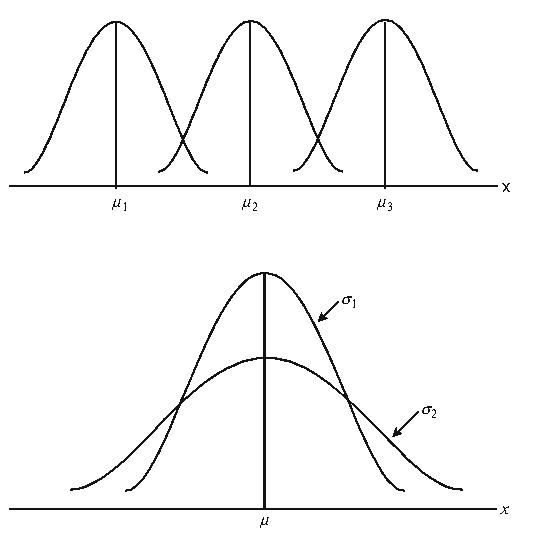
\includegraphics[width=0.40\textwidth]{figures/normal.pdf}
        \end{figure}
    \end{frame}


  \begin{frame}
        \frametitle{Repaso de estad\'istica: Funciones de distribuci\'on}
        \begin{itemize}
            \item \term{Normal univariante}: $x\sim \N(\mu, \sigma^2)$; normal estandarizada: $z\sim \N(0, 1)$
            \item \term{Normal multivariante}: $\mathbf{x}\sim \N(\mu, \Sigma)$ donde $\mathbf{x}:K \times 1$, $\mu:K \times 1$ y $\Sigma:K \times K$.
            \item [] Propiedades:
            \begin{itemize}
                \item  Dada $\mathbf{x}\sim \N(\mu, \Sigma)$ y $a:K \times 1$ entonces  $a'\mathbf{x} \sim \N(a'\mu,a'\Sigma a)$.
                \item Dada $\mathbf{x}\sim \N(\mu, \Sigma)$ y $A:Q \times K$ entonces  $A\mathbf{x} \sim \N(A\mu,A\Sigma A')$.
                \item Dada $\mathbf{x}\sim \N(\mu, \Sigma)$. Entonces $\{x_1,...,x_K\}$ son independientes si y s\'olo si $\Sigma$ es diagonal.
            \end{itemize}
        \end{itemize}
    \end{frame}
    
  \begin{frame}
        \frametitle{Repaso de estad\'istica: Funciones de distribuci\'on}
        \begin{itemize}
            \item Ejemplo: Normal bivariante. Obtener funci\'on de distribuci\'on de $x + y$.
            \item [] Soluci\'on: Sea $\mathbf{x}=(x,y)'\sim \N(\mu,\Sigma)$ con $\mu=(\mu_x,\mu_y)'$ y $\Sigma=\begin{pmatrix}\sigma_x^2 & \sigma_{xy}\\ \sigma_{xy} & \sigma_y^2\end{pmatrix}$. Tomando $a=(1,1)'$, $x+y=a'\mathbf{x}$, y por la propiedad anterior,
            \begin{align*}
            x+y = a'\mathbf{x} \sim \N(a'\mu,\, a'\Sigma a) = \N(\mu_x+\mu_y,\; \sigma_x^2+\sigma_y^2+2\sigma_{xy}).
            \end{align*}
        \end{itemize}
    \end{frame}


  \begin{frame}
        \frametitle{Repaso de \'algebra de matrices}
        \begin{itemize}
            \item Dado $A \geq 0$ (semidefinida positiva) podemos encontrar $B$ tal que $A = B B'$. Llamamos a $B = A ^{1/2}$ (por razones obvias).
            \item Propiedad: $B^{-1}AB'^{-1} = B^{-1}BB'B'^{-1} = I$. Llamamos a $B ^{-1}= A^{-1/2}$.
            \item Para resumir: dado  $A \geq 0$ siempre podemos definir una matriz $A^{-1/2}$ que verifica $A^{-1/2}AA'^{-1/2}=I$.
        \end{itemize}
    \end{frame}

  \begin{frame}
        \frametitle{Ejemplo}
        \begin{itemize}
            \item Ejemplo: Si $\mathbf{x}\sim \N(0, \Sigma)$ entonces   $\Sigma^{-\frac{1}{2}} \mathbf{x}\sim \N(0, I_K)$.
            \item [] Soluci\'on: Tomando $A=\Sigma^{-1/2}$ en la propiedad $A\mathbf{x}\sim \N(A\mu, A\Sigma A')$,
            \begin{align*}
            \Sigma^{-1/2}\mathbf{x} \sim \N\left(\Sigma^{-1/2}\cdot 0,\; \Sigma^{-1/2}\Sigma\Sigma'^{-1/2}\right) = \N(0, I_K),
            \end{align*}
            donde $\Sigma^{-1/2}\Sigma\Sigma'^{-1/2}=I_K$ por construcci\'on de $\Sigma^{-1/2}$ (repaso de \'algebra de matrices).
        \end{itemize}
    \end{frame}


	\begin{frame}
		\frametitle{Ejemplo: Media muestral con varianza muestral}
		\small
		\begin{itemize}
			\item Para $\mathbf{y}:K\times 1$
			\begin{align*}
				\sqrt{N} \widehat{\boldsymbol{\Sigma}}^{-1/2}  \left(\bar{\mathbf{y}} - \boldsymbol{\mu}\right)\dto \N(0,I_K).
			\end{align*}
			donde $\Var(\mathbf{y})=\boldsymbol{\Sigma}$ y $\widehat{\boldsymbol{\Sigma}}\pto\boldsymbol{\Sigma}$.
			\item [] Soluci\'on: Por el TCL, $\sqrt{N}(\bar{\mathbf{y}}-\boldsymbol{\mu})\dto \N(0,\boldsymbol{\Sigma})$. Como $\widehat{\boldsymbol{\Sigma}}\pto\boldsymbol{\Sigma}$ y la ra\'iz inversa es continua, $\widehat{\boldsymbol{\Sigma}}^{-1/2}\pto\boldsymbol{\Sigma}^{-1/2}$ (teorema de la funci\'on continua). Por Slutsky,
			\begin{align*}
			\sqrt{N} \widehat{\boldsymbol{\Sigma}}^{-1/2}  \left(\bar{\mathbf{y}} - \boldsymbol{\mu}\right) \dto \boldsymbol{\Sigma}^{-1/2}\N(0,\boldsymbol{\Sigma}) = \N(0,\boldsymbol{\Sigma}^{-1/2}\boldsymbol{\Sigma}\boldsymbol{\Sigma}'^{-1/2}) = \N(0,I_K),
			\end{align*}
			usando el resultado que vimos anteriormente ($\boldsymbol{\Sigma}^{-1/2}\boldsymbol{\Sigma}\boldsymbol{\Sigma}'^{-1/2}=I_K$).
		\end{itemize}
	\end{frame}

		  		
	% --------------------------------------------------- Slide --
	\subsection{Teorema de la funci\'on continua (para $\dto$.)}
	\begin{frame}
		\frametitle{Teorema de la funci\'on continua (para $\dto$)}
		\begin{itemize}
			\item Si $z_N \dto z$ cuando $N \to \infty$ y $g: \SR^m\to \SR^k$ tiene un conjunto de puntos de discontinuidad $D_g$ tales que $\Pr(z \in D_g)=0$, entonces
			\begin{align*}
			g(z_N) \dto g(z) \text{ cuando }N \to \infty.
			\end{align*}
		\end{itemize}
	\end{frame}

    \begin{frame}
        \frametitle{Repaso de estad\'istica:  Funciones de distribuci\'on}
        \begin{itemize} 
            \item \term{Chi-cuadrado $\chi^2_Q$}
            \item Dadas $\{z_1,...,z_Q\}$ independientes y $z_j\sim \N(0,1)$ entonces $y=\sum_{j=1}^Qz_j^2$ se distribuye como una $\chi^2_Q$.
        \end{itemize}
        \begin{figure}
            \centering
            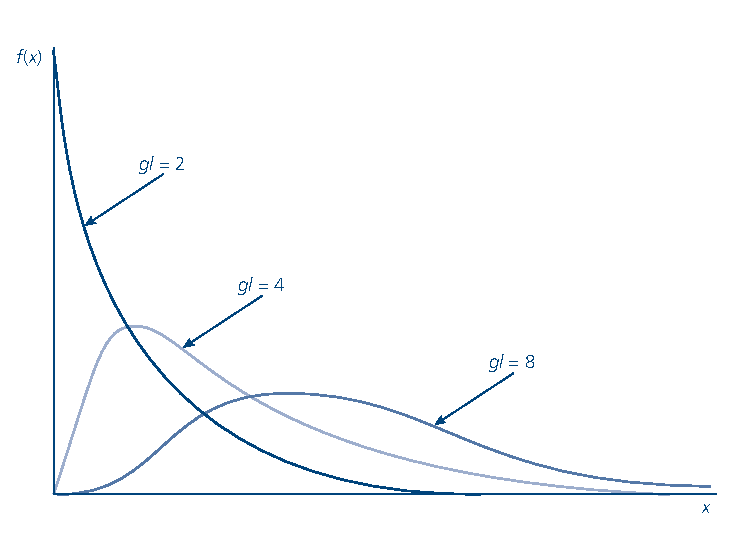
\includegraphics[width=0.50\textwidth]{figures/chi_2.pdf}
        \end{figure}
    \end{frame}

	\begin{frame}
		\frametitle{Ejemplo}
		\begin{itemize}
			\item Para $y$ escalar
			\begin{align*}
				N \frac{(\bar y - \mu)^2}{S^2} \dto \chi^2_1.
			\end{align*}
			\item [] Soluci\'on: Ya vimos $\sqrt{N}(\bar y-\mu)/S \dto \N(0,1)$. La funci\'on $g(x)=x^2$ es continua, luego por el teorema de la funci\'on continua (para $\dto$),
			\begin{align*}
			N\frac{(\bar y-\mu)^2}{S^2}=\left(\sqrt{N}\frac{\bar y-\mu}{S}\right)^2 \dto z^2, \quad z\sim\N(0,1),
			\end{align*}
			y $z^2\sim \chi^2_1$ por definici\'on (suma de un cuadrado de una normal est\'andar).
		\end{itemize}
	\end{frame}


	\begin{frame}
		\frametitle{Ejemplo}
		\small
		\begin{itemize}
			\item Para $\mathbf{y}:K\times 1 $
			\begin{align*}
				N \left(\bar{\mathbf{y}} - \boldsymbol{\mu}\right)' \widehat{\boldsymbol{\Sigma}}^{-1}  \left(\bar{\mathbf{y}} - \boldsymbol{\mu}\right) \dto \chi^2_K.
			\end{align*}
			\item [] Soluci\'on: Sea $\mathbf{w}_N=\sqrt{N}\widehat{\boldsymbol{\Sigma}}^{-1/2}(\bar{\mathbf{y}}-\boldsymbol{\mu})\dto \mathbf{w}\sim\N(0,I_K)$ (que vimos anteriormente). Como $g(\mathbf{z})=\mathbf{z}'\mathbf{z}$ es continua, por el teorema de la funci\'on continua,
			\begin{align*}
			\mathbf{w}_N'\mathbf{w}_N = N(\bar{\mathbf{y}}-\boldsymbol{\mu})'\widehat{\boldsymbol{\Sigma}}^{-1}(\bar{\mathbf{y}}-\boldsymbol{\mu}) \dto \mathbf{w}'\mathbf{w},
			\end{align*}
			usando $\widehat{\boldsymbol{\Sigma}}^{-1/2\prime}\widehat{\boldsymbol{\Sigma}}^{-1/2}=\widehat{\boldsymbol{\Sigma}}^{-1}$, y $\mathbf{w}'\mathbf{w}=\sum_{k=1}^K w_k^2\sim \chi^2_K$ por definici\'on, ya que $w_1,...,w_K$ son independientes $\N(0,1)$.
		\end{itemize}
	\end{frame}

	
% --------------------------------------------------- Slide --
	\subsection{M\'etodo delta}
	\begin{frame}
		\frametitle{M\'etodo delta}
		\begin{itemize}
			\item Si $\sqrt{N}(\hat \theta_N - \theta ) \dto \N(0,V)$ donde $\theta$ es $m\times 1$, y $g(\theta):\SR^m\to \SR^k$ es continuamente diferenciable en la vecindad de $\theta$, entonces cuando $N \to \infty$
			\begin{align*}
			\sqrt{N}(g(\hat \theta_N) - g(\theta) ) \dto \N(0,G'VG),
			\end{align*}
			donde $G(z)=\frac{\partial}{\partial z}g(z)'$ y $G=G(\theta)$.
		\end{itemize}
	\end{frame}
	
	% --------------------------------------------------- Slide --
	\begin{frame}
		\frametitle{Ejemplos}
		\begin{itemize}
			\item \term{Media muestral al cuadrado}: $\bar y^2$
			\begin{align*}
			\sqrt{N} (\bar y^2 - \mu^2) \dto \N(0, 4 \mu^2 \sigma^2).
			\end{align*}
			\item [] Soluci\'on: Por el TCL, $\sqrt{N}(\bar y-\mu)\dto \N(0,\sigma^2)$. Aplicamos el m\'etodo delta con $g(\theta)=\theta^2$, $G=g'(\mu)=2\mu$,
			\begin{align*}
			\sqrt{N}(\bar y^2-\mu^2) = \sqrt{N}(g(\bar y)-g(\mu)) \dto \N(0, G^2\sigma^2) = \N(0, 4\mu^2\sigma^2).
			\end{align*}
			\item [] Nota: Diferencia con la distribuci\'on asint\'otica de $N (\bar y-\mu)^2/S^2 \dto \chi^2_1$.
		\end{itemize}
	\end{frame}
	
	
	% --------------------------------------------------- Slide --
	\begin{frame}
		\frametitle{Ejemplos}
		\small
		\begin{itemize}
			\item <1-> \term{Efecto marginal para cambios grandes de log}
			\item [] <1-> Dado el modelo de regresi\'on $\log y = \beta_0 +\beta_{1} x+ u$ estamos interesados en el efecto marginal de $x$
			\begin{align*}
			\frac{\Delta \E(y|x)}{\E(y|x)} \times 100 \approx [(\exp(\beta_1)-1)  \times 100] \Delta x.
			\end{align*}
			Tenemos un estimador consistente $\hat \beta_1$ que satisface $\sqrt{N}(\hat \beta_1-\beta_1)\dto \N(0, V_{11})$. Proponga un estimador consistente de $(\exp(\beta_1)-1)  \times 100$ y encuentre su distribuci\'on asint\'otica.
			\item <2-> Respuesta: por el m\'etodo delta con $g(\beta_1)=(\exp(\beta_1)-1)\times 100$ y $G=g'(\beta_1)=100\exp(\beta_1)$,
			\begin{align*}
			\sqrt{N}\left[(\exp(\hat \beta_1)-1)\times 100 - (\exp(\beta_1)-1)\times 100\right] \dto \N(0, 10000\exp(2\beta_1) V_{11}).
			\end{align*}
			Estimador consistente: $(\exp(\hat \beta_1)-1)\times 100$ (teorema de la funci\'on continua, $\exp(\cdot)$ es continua).
		\end{itemize}
	\end{frame}
	% --------------------------------------------------- Slide --
	\begin{frame}
		\frametitle{Ejemplos}
		\begin{itemize}
			\item Dado el vector aleatorio $(x_1,\, x_2)$
			con
			\begin{align*}
				\E\left(
				\begin{array} {c}
					x_1 \\
					x_2
				\end{array}
				\right)=
				\left(
				\begin{array} {c}
					\mu_1 \\
					\mu_2
				\end{array}
				\right)
			\end{align*} y
			\begin{align*}
				\Var \left(
				\begin{array} {c}
					x_1 \\
					x_2
				\end{array}
				\right)=
				\left(
				\begin{array} {c c}
					\sigma^2_1 &  \sigma_{12}\\
					\sigma_{12} &  \sigma^2_{2}
				\end{array}
				\right)
			\end{align*}
			?`Cu\'al es la distribuci\'on asint\'otica de $z_N=\log(\bar x_1)+\log(\bar x_2)$
		\end{itemize}
	\end{frame}

	
	
	\begin{frame}
		\frametitle{Ejemplos}
		\begin{itemize}
			\item Dado el vector aleatorio $(x_1,\, x_2)$
			con
			\begin{align*}
			\E\left(
			\begin{array} {c}
			x_1 \\
			x_2
			\end{array}
			\right)=
			\left(
			\begin{array} {c}
			\mu_1 \\
			\mu_2
			\end{array}
			\right)
			\end{align*} y
			\begin{align*}
			\Var \left(
			\begin{array} {c}
			x_1 \\
			x_2
			\end{array}
			\right)=
			\left(
			\begin{array} {c c}
			\sigma^2_1 &  \sigma_{12}\\
			\sigma_{12} &  \sigma^2_{2}
			\end{array}
			\right)
			\end{align*}
			?`Cu\'al es la distribuci\'on asint\'otica de $z_N=\log(\bar x_1)+\log(\bar x_2)$
			\item Respuesta
			\begin{align*}
             \sqrt{N}((\log(\bar x_1)+\log(\bar x_2))-(\log \mu_1+\log \mu_2)) \\
             \dto\N(0,\frac{\sigma_1^2}{\mu_1^2}+\frac{\sigma_2^2}{\mu_2^2}+2\frac{\sigma_{12}}{\mu_1\mu_2})
            \end{align*}
		\end{itemize}
	\end{frame}

	\begin{frame}
		\frametitle{Ejemplos: soluci\'on}
		\small
		\begin{itemize}
			\item Aplicamos el m\'etodo delta a $g(x_1,x_2)=\log(x_1)+\log(x_2)$, con gradiente
			\begin{align*}
			G = \left.\frac{\partial g}{\partial (x_1,x_2)'}\right|_{(\mu_1,\mu_2)} = \left(\frac{1}{\mu_1},\ \frac{1}{\mu_2}\right)'.
			\end{align*}
			\item [] La varianza asint\'otica es
			\begin{align*}
			G'\Sigma G &= \left(\frac{1}{\mu_1},\ \frac{1}{\mu_2}\right)
			\begin{pmatrix}\sigma_1^2 & \sigma_{12}\\ \sigma_{12} & \sigma_2^2\end{pmatrix}
			\begin{pmatrix}1/\mu_1\\ 1/\mu_2\end{pmatrix} \\
			&= \frac{\sigma_1^2}{\mu_1^2}+\frac{\sigma_2^2}{\mu_2^2}+2\frac{\sigma_{12}}{\mu_1\mu_2}.
			\end{align*}
			\item [] Por el m\'etodo delta, $\sqrt{N}(g(\bar x_1,\bar x_2)-g(\mu_1,\mu_2))\dto \N(0,G'\Sigma G)$, que es el resultado de la Respuesta.
		\end{itemize}
	\end{frame}

	% --------------------------------------------------- Slide --
\end{document}